% Created 2021-01-24 Sun 22:50
% Intended LaTeX compiler: pdflatex
\documentclass[11pt]{article}
\usepackage[utf8]{inputenc}
\usepackage[T1]{fontenc}
\usepackage{graphicx}
\usepackage{grffile}
\usepackage{longtable}
\usepackage{wrapfig}
\usepackage{rotating}
\usepackage[normalem]{ulem}
\usepackage{amsmath}
\usepackage{textcomp}
\usepackage{amssymb}
\usepackage{capt-of}
\usepackage{hyperref}
\usepackage{minted}
\hypersetup{colorlinks=true, linkcolor=black, filecolor=red, urlcolor=blue}
\usepackage[turkish]{babel}
\author{Eren Hatırnaz}
\date{22 Eylül 2019}
\title{Yazılım Gündemi - 10\\\medskip
\large 16-22 Eylül 2019}
\hypersetup{
 pdfauthor={Eren Hatırnaz},
 pdftitle={Yazılım Gündemi - 10},
 pdfkeywords={},
 pdfsubject={},
 pdfcreator={Emacs 27.1 (Org mode 9.3)},
 pdflang={Turkish}}
\begin{document}

\maketitle
\tableofcontents \clearpage\shorthandoff{=}

\begin{center}
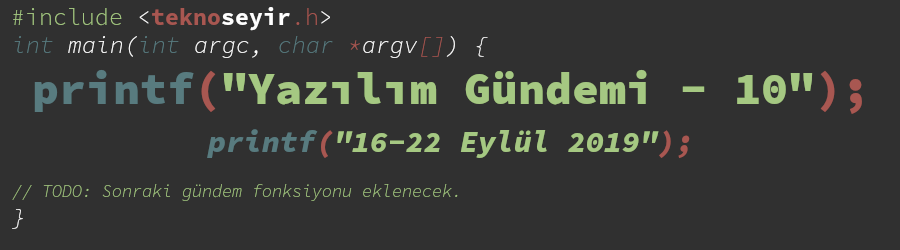
\includegraphics[width=.9\linewidth]{gorseller/yazilim-gundemi-banner.png}
\end{center}

\begin{center}
\href{../09/yazilim-gundemi-09.pdf}{< Önceki Gündem} | \textbf{16-22 Eylül 2019} | \href{../11/yazilim-gundemi-11.pdf}{Sonraki Gündem >}

\href{https://teknoseyir.com/blog/yazilim-gundemi-10-16-22-eylul-2019}{TeknoSeyir'de Oku}
\end{center}

\section{Richard Stallman, Özgür Yazılım Vakfı başkanlığından ve MIT'deki \href{https://www.engadget.com/2019/09/17/rms-fsf-mit-epstein/}{görevinden istifa etti}}
\label{sec:orgb505dee}
Daha doğrusu istifa etmek zorunda kaldı demek daha doğru olur. Çünkü kendisini
hiç sokmaması gereken bir duruma soktu ve artık sonuçlarına katlanmak zorunda.
Olaylar 12 Eylül tarihinde Medium sitesinde yayınlanan \href{https://medium.com/@selamie/remove-richard-stallman-fec6ec210794}{şu blog yazısı} ile
başlıyor. Bu yazıda, Richard Stallman'ın MIT'deki yapay zeka laboratuvarı mail
listesindeki çocuk istismarını savunmaya kadar giden mailleri ifşa edilmiş.
Mailleri aynı zamanda \href{https://assets.documentcloud.org/documents/6405929/09132019142056-0001.pdf}{buradan da} okuyabilirsiniz. Bunlar ortaya çıkınca doğal
olarak herkes Stallman'ın üzerine gitmeye başladı ve sonuç \href{https://www.fsf.org/news/richard-m-stallman-resigns}{bu şekilde} oldu.

Olaylar hakkında fazla detaya girmeyeceğim zaten internet üzerinde hem
İngilizce hem de Türkçe olarak birçok kaynakta yer aldı(*). Bu haftaki gündem
değerlendirmesinde \href{https://youtu.be/aRo4U0scAI4?t=1546}{Murat Abi de değindi}. Detayları oralardan okuyabilir ya da
dinleyebilirsiniz.

Ben de özgür yazılım destekçisi birisiyim fakat Stallman'ın politik görüşlerini
pek takip etmiyorum. Web sitesindeki \href{https://stallman.org/archives/2019-jul-oct.html}{şu sayfaya} baktığımda buna benzer
düşünceleri daha önce de dile getirdiğini gördüm. Bu tarz uçlarda dolaşmayı
seven birisi olduğu açık fakat bu olayın savunulacak hiçbir yanı yok -sonradan
yaptığının yanlış olduğunun farkına varmış olsa bile.

Ayrıca Richard Stallman'ın Özgür Yazılım Hareketi adına \href{https://sfconservancy.org/news/2019/sep/16/rms-does-not-speak-for-us/}{konuşma yapması da
yasaklandı}. Açıkcası her ne kadar hareketin kurucusu olsa bile Richard
Stallman'ın ilahlaştırılmayıp, savunulmaya çalışılmaması beni sevindirdi. Bu
demek oluyor ki, Özgür Yazılım Hareketi Richard Stallman olmadan da devam
edebilir.

\textbf{Kaynaklar}:
\begin{itemize}
\item \href{https://www.bilimma.com/richard-stallman-cocuk-istismarini-savundu/}{Richard Stallman çocuk istismarını savundu – Bilimma Bilim Haberleri}
\item \href{https://www.vice.com/en\_us/article/mbm74x/computer-scientist-richard-stallman-resigns-from-mit-over-epstein-comments}{Computer Scientist Richard Stallman Resigns From MIT Over Epstein Comments - \ldots{}}
\item Reddit tartışmaları:
\begin{itemize}
\item \href{https://www.reddit.com/r/programming/comments/d59r46/richard\_stallman\_resigns\_from\_mit\_over\_epstein/}{Richard Stallman Resigns From MIT Over Epstein Comments : programming}
\item \href{https://www.reddit.com/r/programming/comments/d5art6/richard\_m\_stallman\_resigns\_free\_software/}{Richard M. Stallman resigns — Free Software Foundation : programming}
\end{itemize}
\end{itemize}
\section{Bir geliştirici ABD Göçmenlik ve Gümrük Muhafaza kurumunu \href{https://www.zdnet.com/article/developer-takes-down-ruby-library-after-he-finds-out-ice-was-using-it/}{protesto etti}}
\label{sec:orgebe1633}
\href{https://github.com/sethvargo}{Seth Vargo} isimli geliştirici, kişisel projelerinin birinin, dolaylı bir yoldan
ABD Göçmenlik ve Gümrük Muhafaza kurumuyla yapılan bir iş anlaşmasına dahil
olması nedeniyle ilgili projesini her yerden kaldırdı.

Şu an Google'da mühendis olarak çalışan bu arkadaş, eskiden \href{https://www.chef.io/}{Chef} isimli bir
şirkette çalışıyormuş ve o zamanlarda \href{https://github.com/sethvargo/chef-sugar}{Chef Sugar} isimli kişisel bir proje
geliştirip, GitHub hesabında ve RubyGems sitesinde paylaşmış. Daha sonra da
ilgili kütüphane, Chef'in bağımlılıkları (dependency) arasına girmiş.

Bu haftanın başlarında \href{https://twitter.com/shanley/status/1173692656192385024}{Twitter'da bir kullanıcı}nın Chef şirketi ile ABD
Göçmenlik ve Gümrük Muhafaza kurumunun yaptığı 95.500\$'lık anlaşmayı ortaya
çıkarınca, kütüphanenin geliştiricisi de kurumu protesto etmek için ilgili
kütüphanenin kodlarını GitHub'dan ve RubyGems sitesinden sildi. Bu durumdan
etkilenen projeler de olmuş haliyle. Protesto nedeni olarak da "insanlık dışı
muamele, temel insan haklarının reddi" vb. gibi konuları göstermiş. İlgili
kurum hakkında pek bilgim yok ama söz konusu Amerika olunca geliştiriciye hak
veresim geliyor.

Geliştirici bunu protesto amacıyla yapmış fakat kodları açık kaynak bir lisans
ile paylaştığı için haliyle Chef şirketi de eski kodları bulup, tekrar kendi
hesaplarına yüklemişler. Yine de ilginç bir protesto yöntemi olarak tarihe not
düşmüş oldu.
\section{GitHub, Semmle isimli \href{https://github.blog/2019-09-18-github-welcomes-semmle/}{şirketi satın aldı}}
\label{sec:org5aaae3f}
\href{https://semmle.com/}{Semmle}, bir semantik kod analizi motoru. Yani kodlarınızı analiz edip, olası
güvenlik zafiyetlerini ya da daha önce keşfedilmiş güvenlik açıklarını CVE
numaraları ile birlikte sunan bir hizmet. Daha çok firmalardaki güvenlik
takımındaki geliştiriciler tarafından kullanılan bir servis.

GitHub da bu şirketi satın alarak bünyesine kattı ve artık GitHub ile daha
entegre olacağı hatta direkt GitHub'ın içerisinde bir servis olarak
kullanılabileceği \href{https://venturebeat.com/2019/09/18/github-acquires-semmle-to-help-developers-spot-code-exploits/}{yönünde görüşler var}. Bakalım önümüzdeki aylarda mutlaka bir
kullanım senaryosu olarak karşımıza çıkarır bunu GitHub.
\section{Chrome 78 Beta ile \href{https://blog.chromium.org/2019/09/chrome-78-beta-new-houdini-api-native.html?m=1}{gelen API yenilikleri}}
\label{sec:org01b86fe}
19 Eylül günü yayınlanan bu chrome sürümü ile API sistemine bazı yenilikler
gelmiş. Şöyle ki:

\subsection{Özel CSS özellikleri ve değişkenler}
\label{sec:orgce9c8da}
W3C organizasyonunun \href{https://drafts.css-houdini.org/}{CSS-TAG Houdini} ekibi tarafından oluşturulmuş bu
özellik sayesinde artık CSS tarafında kendimize özel css özellikleri
oluşturabileceğiz. Yani bu şekilde:
\begin{minted}[breaklines=true,breakanywhere=true,frame=lines, linenos, label=JavaScript, labelposition=topline]{javascript}
window.CSS.registerProperty({
  name: '--my-color',
  syntax: '<color>',
  inherits: false,
  initialValue: 'black',
});
\end{minted}
JavaScript tarafında özelliği tanımladıktan sonra, CSS tarafında böyle
kullanabileceğiz:
\begin{minted}[breaklines=true,breakanywhere=true,frame=lines, linenos, label=CSS, labelposition=topline]{css}
.thing {
    --my-color: red;
}
\end{minted}
Front-End tarafına pek yakın birisi olmadığım için kullanım senaryosunu
çözemedim ama \href{https://web.dev/css-props-and-vals/}{buradaki sayfadan} daha detaylı bilgiler alabilirsiniz.
\subsection{Dosya sistemine erişim}
\label{sec:orgf612b12}
Bu özelliğin geleceğini daha önceki yazılım gündemi yazısında (bkz: \href{../07/yazilim-gundemi-07.pdf}{Yazılım
Gündemi - 7}) söylemiştim. Bu sürümde, Chrome'a eklenen Origin Trials
özelliği üzerinden aktifleştirilebilir olmuş. Yani artık buna göre kodlanan
siteler sizin seçtiğiniz bir dosyaya doğrudan erişip üzerinde, okuma-yazma
işlemleri yapabilecek. İlgili yazıda bu özelliğin kullanım alanı için
Google, çevrim içi uygulamalar (resim\&video düzenleme, metin editörü vb.) bu
özellik sayesinde daha kolay kullanılabilecek demiş. Önceden de bu tarz
siteleri kullanabiliyorduk fakat orada site sadece dosyayı okuyabiliyordu.
Mesela bir resimde değişiklik yaptığınızda o tarayıcıda kalıyordu, kaydet
dediğinizde farklı bir dosya olarak indiriliyordu, artık siteler doğrudan
dosyayı değiştirebilecekler. Bana kötüye kullanımı çok mümkün bir özellik
gibi geliyor, ben şahsen o şekilde bir izini hiçbir siteye vermem. Siz ne
düşünüyorsunuz bu özellik hakkında? Yorumlar kısmında konuşalım.

API sistemindeki diğer değişiklikler için konu bağlığına eklediğim bağlantıya
tıklayabilirsiniz.
\section{Safari 13 ile \href{https://developer.apple.com/documentation/safari\_release\_notes/safari\_13\_release\_notes}{gelen API yenilikleri}}
\label{sec:org8028c3d}
Bu hafta iOS 13 ile birlikte yayınlanan Safari 13'de yeni API özellikleri
mevcut. Bunlardan bazıları şu şekilde:
\begin{itemize}
\item Web siteler artık telefonun karanlık moda geçtiğini anlayıp kendilerini de
karanlık temaya geçirebilecekler.
\item "Apple ile Giriş Yap" özelliği web sitelere eklenebilecek
\item Sayfada yer alan \texttt{iframe} ler artık sayfayı değiştiremeyecek.
\item Koni şeklinde CSS renk geçişleri (gradient) için destek.
\item JavaScript artık daha az bellik kullanıyor.
\item \texttt{\_\_Secure-} ve \texttt{\_\_Host-} çerez ön-ekleri için destek.
\item Apple Pay için destek
\end{itemize}

API sistemindeki diğer değişiklikler için konu bağlığına eklediğim
bağlantıya tıklayabilirsiniz.
\section{Microsoft programcılar için yeni \href{https://devblogs.microsoft.com/commandline/cascadia-code/}{yazı stilini duyurdu}: \href{https://github.com/microsoft/cascadia-code}{Cascadia Code}}
\label{sec:orge422b45}
\begin{center}
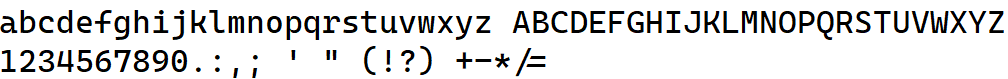
\includegraphics[width=.9\linewidth]{gorseller/cascadia-code-characters.png}
\end{center}

Microsoft, terminal ve programlama araçlarında kullanılmak üzere bu yeni yazı
stilini \href{https://scripts.sil.org/cms/scripts/page.php?site\_id=nrsi\&id=OFL}{SIL Open Font License} isimli lisans ile açık kaynak şekilde duyurdu.
Ben şu an geliştirilmekte olan Windows Terminal uygulamasının da varsayılan
olarak bu yazı stilini kullanacağını tahmin ediyorum. Ben uzun zamandır \href{https://input.fontbureau.com/}{Input
Mono} kullanıyorum ama belki bir ara bunu da deneyebilirim.

\url{gorseller/programming-ligatures.gif}
\section{Etkinlik duyurusu: \href{https://www.qt.io/events/ultimate-graphical-performance-on-stm32-microcontrollers-with-qt-for-mcus-1568631867}{Ultimate Graphical Performance on STM32 microcontrollers with Qt for MCUs}}
\label{sec:orge51111b}
Geçtiğimiz haftalarda tanıtılan Mikroişlemciler için Qt kütüphanesinin tanıtım
etkinlikleri devam ediyor. 25 Eylül tarihinde de bir Webiner (sanal seminer)
düzenlenecekmiş. İlgili arkadaşlar konu başlığına eklediğim bağlantıya
tıklayarak kayıt olabilirler.

\href{https://www.qt.io/events/ultimate-graphical-performance-on-stm32-microcontrollers-with-qt-for-mcus-1568631867}{Etkinlik sayfası}
\section{Diğer Haberler}
\label{sec:org6d2fc21}
\begin{itemize}
\item Microsoft, kendi C++ Standart Kütüphanesini \href{https://devblogs.microsoft.com/cppblog/open-sourcing-msvcs-stl/}{açık kaynak yaptı}: \href{https://github.com/microsoft/STL}{STL}.
\item Modern C kitabının ikinci baskısı Creative-Common lisansı ile \href{https://gustedt.wordpress.com/2019/09/18/modern-c-second-edition/}{çevrim içi
olarak yayınlandı}.
\item KDAB Group, içerisinde çeşitli C++ araçlarının olduğu \href{https://www.kdab.com/introducing-kdtoolbox/}{depoyu açık kaynak
yaptı}: \href{https://github.com/KDAB/KDToolBox}{KDToolbox}.
\item C programlama dilinde asenkron süreçler yönetmeye yarayan \href{https://higherlogics.blogspot.com/2019/09/asynch-asynchronous-stackless.html}{kütüphane açık
kaynak olarak yayınlandı}: \href{https://github.com/naasking/async.h}{async.h}
\item Go için önbellek kütüphanesi \href{https://blog.dgraph.io/post/introducing-ristretto-high-perf-go-cache/}{açık kaynak olarak yayınlandı}: \href{https://github.com/dgraph-io/ristretto}{ristretto}.
\item Neo4j, yeni bir sorgu dili duyurdu: \href{https://neo4j.com/press-releases/query-language-graph-databases-international-standard/}{GQL (Graph Query Language)}
\item Eclipse \href{https://www.eclipse.org/eclipseide/2019-09/noteworthy/}{2019-09 sürümü yayınlandı}.
\begin{itemize}
\item Eclipse IDE 2019-09'a Java 13 desteği kazandıran araç \href{https://marketplace.eclipse.org/content/java-13-support-eclipse-2019-09-413}{Eclipse
Marketplace'de yerini aldı}.
\end{itemize}
\item Kubernetes \href{https://kubernetes.io/blog/2019/09/18/kubernetes-1-16-release-announcement/}{1.16 sürümü duyuruldu}.
\item LLVM \href{http://lists.llvm.org/pipermail/llvm-dev/2019-September/135304.html}{9.0.0 sürümü yayınlandı}.
\item Memcached \href{https://github.com/memcached/memcached/wiki/ReleaseNotes1518}{1.5.18 sürümü duyuruldu}.
\item OpenJDK \href{https://openjdk.java.net/projects/jdk/13/}{13 sürümü yayınlandı}.
\item HgLab \href{https://hglabhq.com/blog/2019/9/19/hglab-1-14-released}{1.14 sürümü yayınlandı}.
\item YugaByteDB \href{https://blog.yugabyte.com/announcing-yugabyte-db-2-0-ga-jepsen-tested-high-performance-distributed-sql/}{2.0 GA sürümü yayınlandı}.
\item NeoVIM \href{https://github.com/neovim/neovim/releases/tag/v0.4.0}{0.4.0 sürümü yayınlandı}, \href{https://github.com/neovim/neovim/commit/e2cc5fe09d98ce1ccaaa666a835c896805ccc196}{Değişiklik Notları}.
\item TextMate \href{https://github.com/textmate/textmate/releases/tag/v2.0}{v2.0 sürümü yayınlandı}.
\item Akademik Çalışmalar:
\begin{itemize}
\item \href{https://arxiv.org/abs/1909.07528}{Emergent Tool Use From Multi-Agent Autocurricula}, \href{https://openai.com/blog/emergent-tool-use/}{Alternatif Kaynak}.
\item \href{https://arxiv.org/abs/1909.08723}{Espresso: A Fast End-to-end Neural Speech Recognition Toolkit}
\end{itemize}
\end{itemize}
\section{Lisans}
\label{sec:orgbe272f9}
\begin{center}
\begin{center}

\includegraphics[height=1.5cm]{../../../img/CC_BY-NC-SA_4.0.png}
\end{center}

\href{yazilim-gundemi-10.pdf}{Yazılım Gündemi - 10} yazısı \href{https://erenhatirnaz.github.io}{Eren Hatırnaz} tarafından \href{http://creativecommons.org/licenses/by-nc-sa/4.0/}{Creative Commons
Atıf-GayriTicari-AynıLisanslaPaylaş 4.0 Uluslararası Lisansı} (CC BY-NC-SA 4.0)
ile lisanslanmıştır.
\end{center}
\end{document}
